\documentclass[12 pt]{report}
\usepackage[spanish, mexico]{babel}
\usepackage[T1]{fontenc}
\usepackage[margin=2.5cm]{geometry}
\usepackage[export]{adjustbox}
\usepackage{caption}
\usepackage{subcaption}
\usepackage{graphicx}
\usepackage{listings}
\usepackage{minted}
\usepackage{fancyhdr}
\usepackage{hyperref}

\graphicspath{ {extras/} }
\usemintedstyle{friendly}
\pagestyle{fancy}
\fancyhf{}
\rhead{\leftmark}
\lhead{Proyecto}
\rfoot{Page \thepage}

\hypersetup{
    colorlinks=true,
    linkcolor=blue,
    filecolor=magenta,      
    urlcolor=cyan,
    pdftitle={Reporte},
    }
\begin{document}
\thispagestyle{empty}

\begin{figure}[ht]
  \minipage{0.76\textwidth}
  
\includegraphics[height = 4.9cm ]{extras/Logo_IPN.png}
  \label{EscudoIPN}
  \endminipage
  \minipage{0.32\textwidth}
  
\includegraphics[height = 4.9cm ,width=4cm]{extras/Logo_ESCOM.png}
  \label{EscudoESCOM}
  \endminipage
\end{figure}

\begin{center}
  \vspace{0.8cm}
  \LARGE
  INSTITUTO POLITÉCNICO NACIONAL
  
  \vspace{0.8cm}
  \LARGE
  ESCUELA SUPERIOR DE COMPUTO
  
  \vspace{1.5cm}	
  \Large
  \textbf{Proyecto final: lineas de producción}

  \vspace{1.0cm}
  \normalsize	
  Los últimos:  \\
  \vspace{.3cm}
  \large
  \textbf{Torres Trejo Victor Federico \\ Sotelo Padrón Lara Leilani \\ Sánchez Flores Guillermo}
  
  \vspace{1cm}
  \normalsize	
  PROFESOR \\
  \vspace{.3cm}
  \large
  \textbf{Edgardo Adrián Franco Martínez}

  \vspace{1cm}
  \normalsize	
  ASIGNATURA \\
  \vspace{.3cm}
  \large
  \textbf{Análisis y Diseño de Algoritmos\\}
  
  \vspace{1cm}
  \today
\end{center}

\tableofcontents

\chapter{Planteamiento del algoritmo y solución}
\section{Problema planteado}
Existe una fabrica de automóviles que tiene dos lineas de montaje, cada una con n estaciones.

Una estación se indica con los sub-índices i j donde i es 1 o 2 que es la linea de montaje en la se encuentra dicha estación y j es el numero de la estación, cada tiempo se indica entonces por a[i][j]. Cada estación tiene un trabajo especifico, por lo que cada chasis de automóvil debe pasar por cada una de las n estaciones para salir de la fábrica. Las estaciones paralelas en cada linea realizan el mismo trabajo. Después de pasar por estación i j, el chasis continua a la estación i (j+1) a menos que se decida transferirse a otra linea.

El continuar en la misma linea no tiene un costo adicional, pero transferirse de la linea i en la estación ($j-1$) a la otra linea en la estación j lleva un tiempo denotado por t[i][j]. Cada linea de montaje tiene su tiempo de entrada e[i] y un tiempo de salida x[i] que pueden ser distintas para las dos lineas.
\section{Solución en fuerza bruta}
La solución en bruta implica explorar todos las rutas posibles que pueda seguir el chasis de automóvil, al final tenemos $2^n$ resultados posibles y comparamos entre todos para ver con cual nos quedamos. El código se ve de la siguiente manera:
\inputminted[firstline = 25, lastline=37]{C}{../solucionBruta.c}

Y se llama a la función de la siguiente manera:
\inputminted[firstline = 46, lastline=46]{C}{../solucionBruta.c}

El inconveniente de esta solución es que tenemos que explorar todas las rutas posibles, aun que no tiene sentido hacerlo se exploran hasta llegar al final del camino, esto tanto en computación como en la vida real es muy cansado e innecesario de realizar, es por ello que se emplea una solución usando Programación Dinámica.
\section{Solución en Programación Dinámica}
Viendo que la solución en fuerza bruta es muy tardada, tratamos de usar el concepto de ''memoización'' para no explorar todas las soluciones. Para usar esta técnica nos apoyamos en un dos arreglos de tamaño n, en cada casilla vamos guardando el mejor camino para ese punto de la estación desde la estación 1 hasta la n. Esto se hace obteniendo que camino nos sale mas barato, si seguir en la linea actual o desde la otra linea cambiarnos a la que estamos analizando, una vez obtenido el mínimo de estas dos, se guardan en la tabla y continuamos, en la siguiente iteración preguntamos si el camino acumulado para llegar a la estación $i-1$ es mejor seguir o de la estación $(i-1)$ de la otra linea es mejor cambiarnos a la actual, esto lo hacemos para todas las estaciones posibles para ambas lineas, de tal manera que en ambas casillas $(n-1)$ se tiene el mejor camino posible para ambas lineas, al final se devuelve el camino mínimo entre estas dos casillas sumándole el tiempo de salida. Como podemos apreciar este algoritmo tardara n veces, y si nosotros comparamos una función gráficamente de $2^n$ vs $n$ claramente es mejor la lineal, y es por ello que la solución en Programación dinámica es mas eficiente. Ademas que es parecido a lo que haría una persona en resolver este problema sin el uso de la computación. Comparar si es mejor quedarse o cambiarse e ir usando esas soluciones para armar una general, que es el concepto de la programación dinámica. Cabe destacar que esto es un enfoque top-down.

\inputminted[firstline = 26, lastline=37]{C}{../solucionDp1.cpp}

Ahora podemos ver que solo usamos la $(i-1)$ casilla para armar la siguiente solución, por lo que visto desde la complejidad espacial que es el uso de memoria, las demás casillas pueden ser innecesarias después de 2 iteraciones, por ello usando 4 variables nosotros almacenamos ese mejor camino para la primer y segunda linea, posteriormente ese lo usamos para calcular el de la mejor linea de la siguiente estación y una vez que ya construimos esa solución, actualizamos los valores para volver a usarlo en la siguiente iteración. En esta solución vemos que solo usamos 4 variables en lugar de 2n, por lo que este código es mas eficiente en cuestión de memoria.
\inputminted[firstline = 17, lastline=28]{cpp}{../solucionDp2.cpp}
\section{Tecnologías web}
Para poder representar la animación web no se hizo uso de ninguna librería de animación web, se hizo el uso de los conceptos de funciones asíncronas y \textbf{await} para resolver la animación. Esto debido a que necesitábamos que el carro se moviera a cierta ''posición'' en la pagina vista como un tablero. Por lo que transportar el carro era sencillo, solo es modificar cuestiones de propiedades de estilos de cada elemento, pero darle la sensación de animación es lo complicado, por ello es que donde entra await, esta función en JavaScript hace que el programa se espere hasta que la promesa responda y devuelva su resultado. Esta promesa devuelve su resultado una vez que la función \textbf{setTimeout} haya concluido, esta función espera una cantidad de segundos dados y ejecuta su porción de código una vez que se cumplió el tiempo establecidos en mili-segundos.

En resumen con el uso de await lo que logramos es que el código espere unos segundos para seguirse ejecutando, con ello movemos el carro lentamente y con la función sleep y el uso de await le damos pausa y un sentido de movimiento, ya que se mueve varias veces en una instrucción. Como en si el await solo funciona en funciones async, se tuvo que hacer la mayoría del código en funciones async para darle ese sentido de mono hilo, también para dar pausas entre movimientos usamos el await sleep. En si en esto consiste nuestra animación, modificaciones con el uso de DOM a los objetos del html y el uso de async/await para lograr esa percepción de movimiento.

Esta es la función sleep desarrollada:
\inputminted[firstline = 117, lastline = 119]{js}{../PaginaWeb/js/main.js}
Y la función que logra animar cierto coche:
\inputminted[firstline = 121, lastline = 149]{js}{../PaginaWeb/js/main.js}
\chapter{Representación del algoritmo}
\section{Bocetos}
\subsection{Solución en fuerza bruta}
Para la solución bruta la animación fue sencilla de proponer o diseñar, es solo crear el dibujo de las lineas de producción con sus respectivas estaciones e ir haciendo mover todos los carros, para que al final se calcularan los $2^n$ resultados y pudiéramos ver cual era el optimo. Cada carro conforme visitaba los nodos se iba a actualizar su valor.
\begin{figure}[h!]
  \centering
  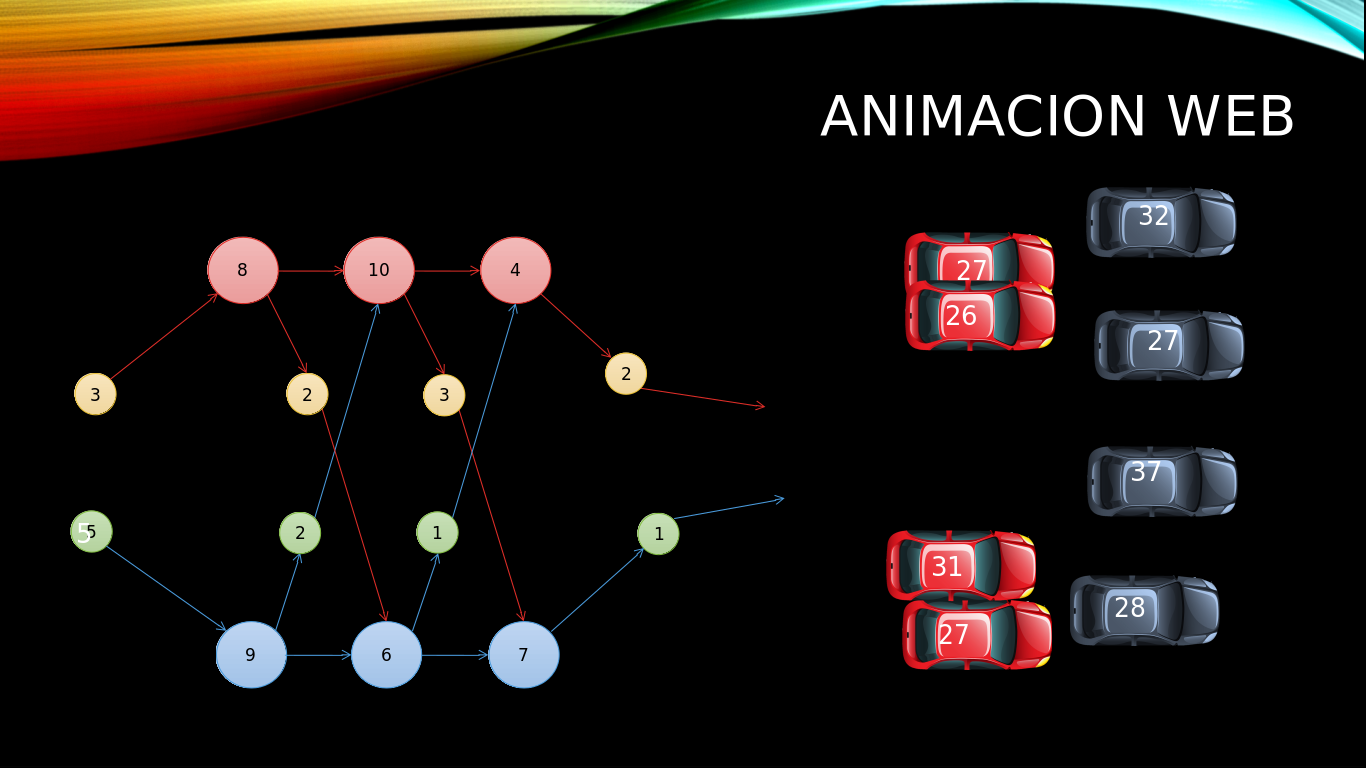
\includegraphics[scale = 0.3]{brutaAnim}
  \caption{Boceto de la animación de la fuerza bruta}
\end{figure}

\subsection{Solución en Programación dinámica}
Para la solución en DP iba a ser similar a la bruta, porque al final si explora ciertas soluciones pero no todas, por lo que solo era cuestión de ver cual era el mejor camino para así generar, eliminar y mover los carros, para esto había solo 4 casos:
\begin{enumerate}
\item ambos carros se quedaran en su linea, entonces avanzaban sin problema
\item el carro de la linea 1 se quedara ahí y para la linea 2 trajéramos el de la linea 1, que era duplicar el carro de la linea 1 y remover el actual de la 2
\item El carro de la linea 2 siguiera en su linea pero el de la linea 1 se tenía que traer desde la 2, por lo que eliminamos el carro actual de la 1 y duplicamos el de la 2 para llevar el duplicado a la 1.
\item Por ultimo era que para ambas lineas teniamos que cambiar de linea, por lo que se eliminaban y duplicaban ambos carros y se cambiaban de linea cada duplicado.
\end{enumerate}
Una vez esto cuando salimos del ciclo for, llevamos los carros al final de la estación, y por ultimo eliminamos el que mas tiempo tardo.
\begin{figure}[h!]
  \centering
  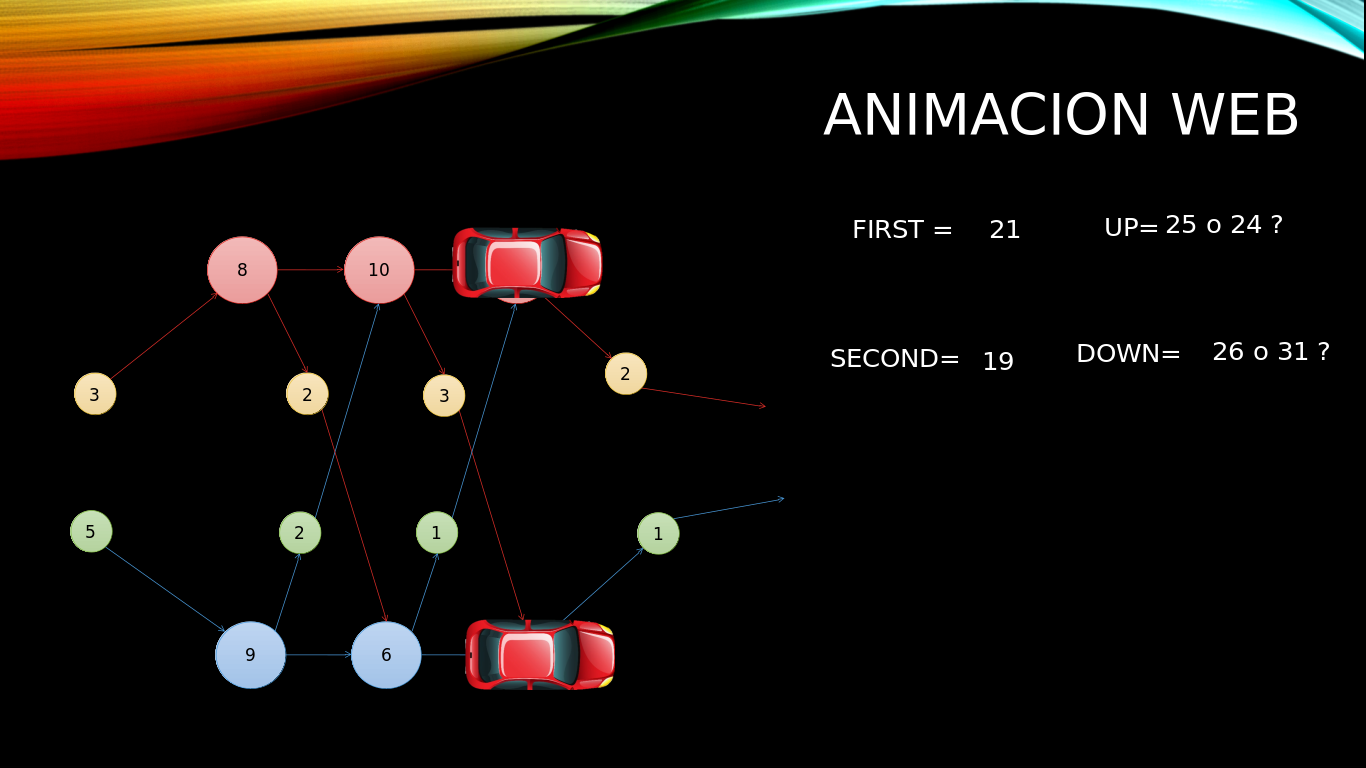
\includegraphics[scale = 0.3]{dpAnim}
  \caption{Boceto de la animación de Programación dinámica}
\end{figure}

\chapter{Pruebas}
\begin{figure}[h!]
  \centering
  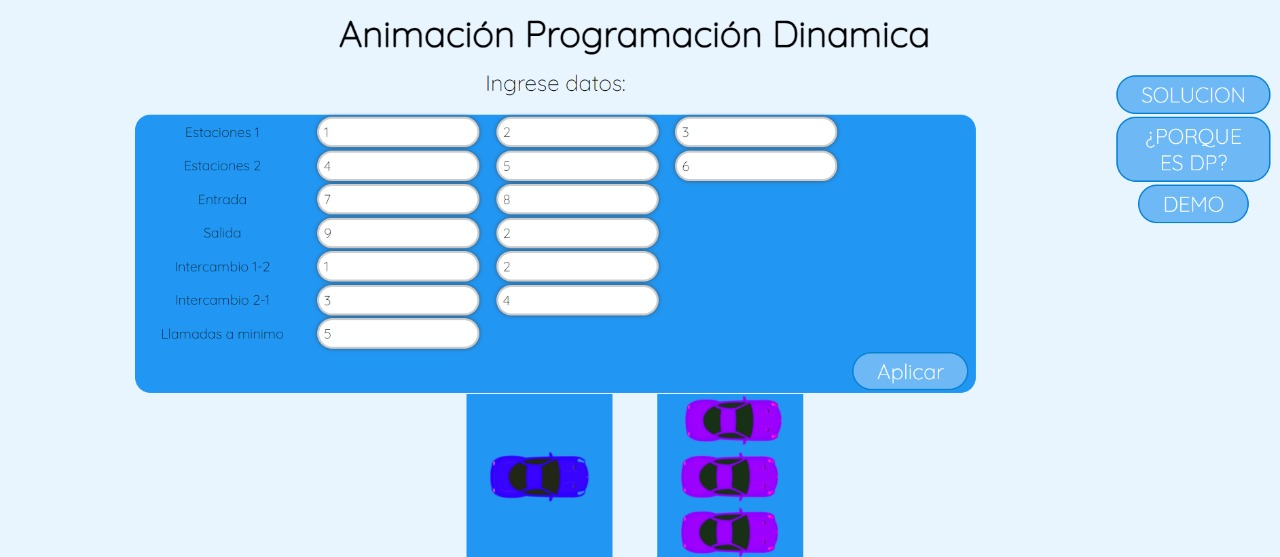
\includegraphics[scale = 0.4]{paginadp1}
  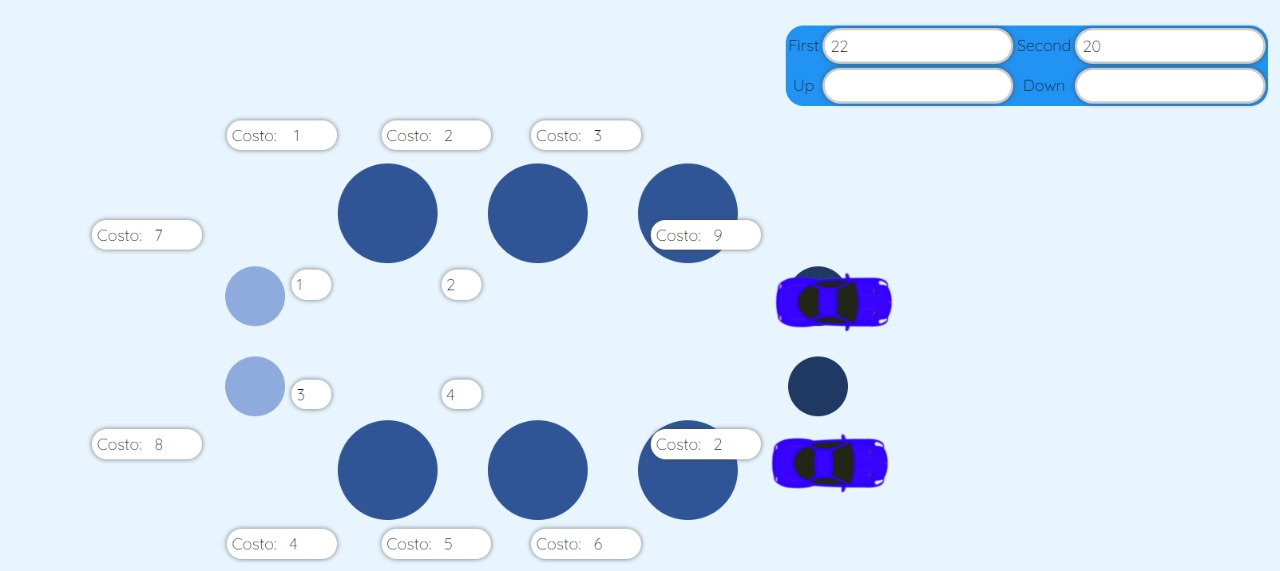
\includegraphics[scale = 0.4]{paginadp2}
\end{figure}
\begin{figure}[h!]
  \centering
  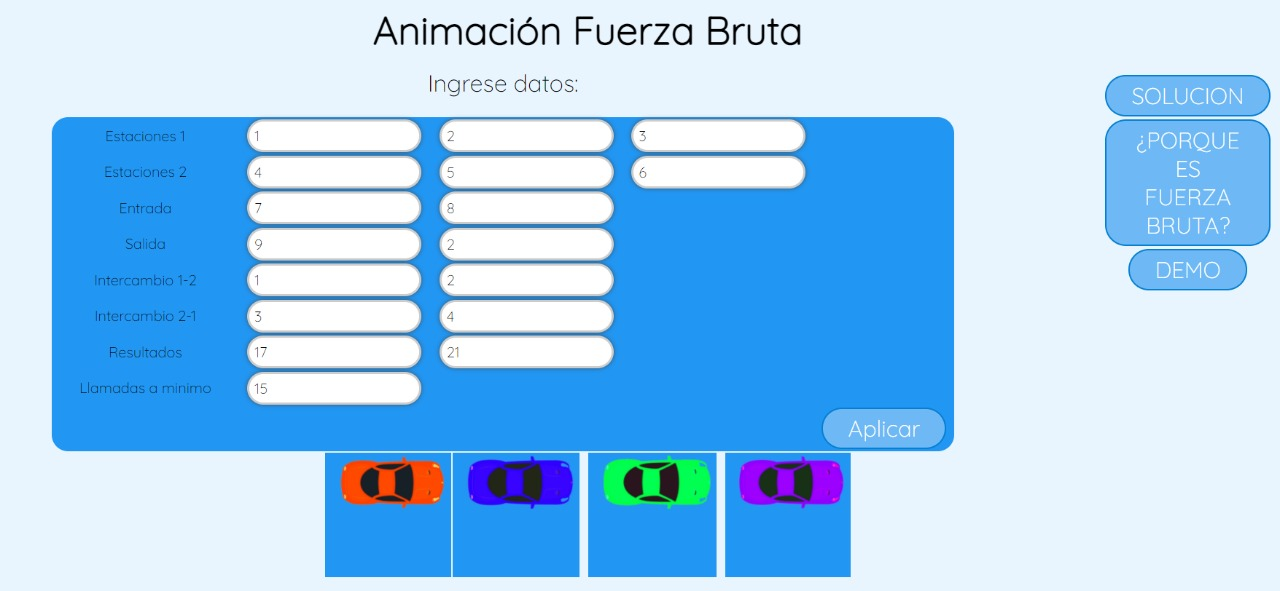
\includegraphics[scale = 0.4]{paginafb1}
  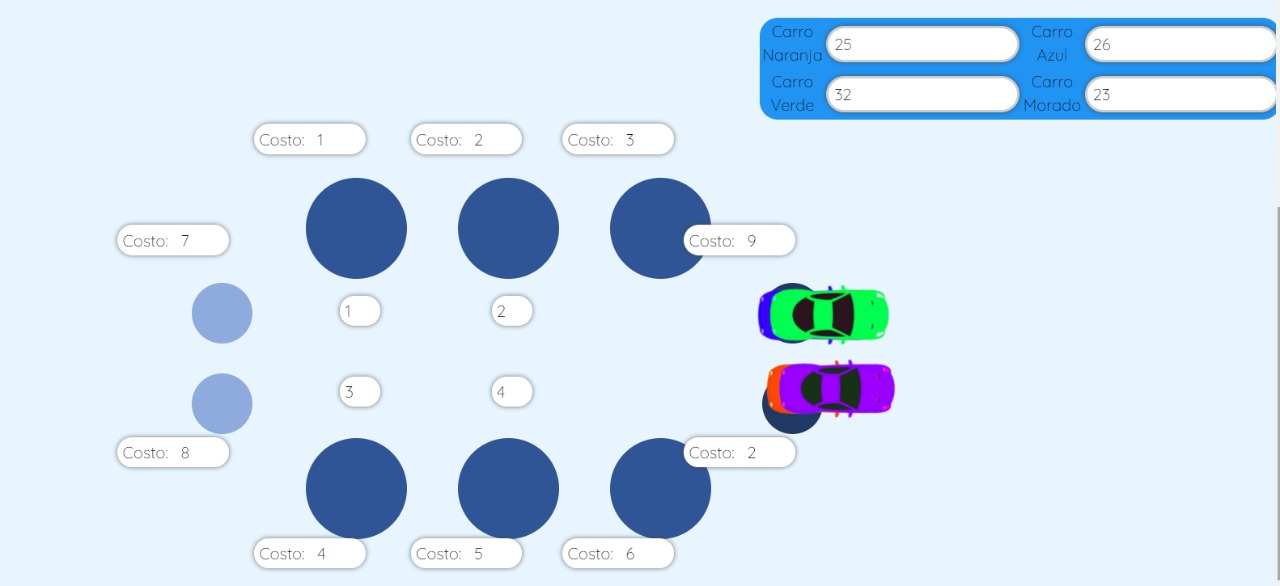
\includegraphics[scale = 0.4]{paginafb2}
\end{figure}

\chapter{Anexos}
\section{Código en fuerza bruta con C}
\inputminted{C}{../solucionBruta.c}
\section{Código en Programación Dinámica con C++}
\inputminted{cpp}{../solucionDp2.cpp}
\section{Código en JavaScript}
\subsection{Código para la Fuerza bruta}
\inputminted{js}{../PaginaWeb/js/main.js}
\subsection{Código para la Programación dinámica}
\inputminted{js}{../PaginaWeb/js/dp.js}
\end{document}
%%% Local Variables:
%%% mode: latex
%%% TeX-master: t
%%% End:
